%!TEX root = /Users/manunavjeevan/Desktop/Research/ML + Lasso/Annotated Literature Review/litNotesML.tex

\section{Deep Learning in NPR \textit{\small Benedikt Bauer and Michael Kohler (AOS, 2019)}}
\label{sec:dl_npr}
Full paper title is ``On Deep Learning As A Remedy for the Curse of Dimensionality in Nonparametric Regression'' and can be found via the AoS website 
\href{https://projecteuclid.org/download/pdfview_1/euclid.aos/1558425645}{here}.

\subsection{Introduction}

In regression analysis, a random vector $(X,Y)$ with values in $\mathbb{R}^d \times \mathbb{R}$ satisfying $\mathbf{E}Y^2 < \infty$ is considered, and an estimation of the relationship between $X$ and $Y$ is attempted. Generally the aim is to minimize the MSE or $L_2$r risk. So the construction of a measurable function $m^*: \mathbb{R}^d \rightarrow \mathbb{R}$ satisfying 
\[m^* =\argmin_{f: \mathbb{R}^d \rightarrow \mathbb{R}} \mathbf{E}\left\{\left|Y- f(X)\right|^2\right\}\]
is of interest. In the following, let $m:\mathbb{R}^d \rightarrow \mathbb{R}$, $m(x) = \mathbf{E}\{Y|X=x\}$ denote the ``regression function''. It is true that for any $f$:
\[\mathbf{E}\left[ \left|Y-f(X)\right|^2\right] = \mathbf{E}\left[\left|Y - m(X)\right|^2\right] + \int \left| f(x) - m(x) \right|^2 \mathbf{P}_X(dx) \]
it is the optimal predictor $m^*$. Moreover, a good estimate $f:\mathbb{R}^d \rightarrow \mathbb{R}$ (in the $L_2$ risk minimization sense) has to keep the ``$L_2$'' error small 
\[\int \left|f(x) - m(x)\right|^2 \mathbf{P}_X(dx)\]
In applications, the distribution of $(X,Y)$ and $m$ are (typically) unkown, but the statistician does have access to a set of data 
\[\mathscr{D}_n = \{(X_1,Y_1), \dots, (X_n, Y_n)\}\]
Goal is typically to create estimates of $m$, $m_n$ to minimize the $L_2$ error. In non-parametric regression estimation of the regression function does not reduce to estimation of finitely many parameters. Gyordi et al. (2002) provide a systematic overview of different approaches and nonparametric estimation results.

\subsubsection{Rate of Convergence}
Well known that one has to restric the class of regression functions one considers to obtain useful results for the rate of convergence. Following definiton of $(p,C)$-smoothness is to that end
\begin{definition}
\label{def:DLNPR-1}
($(p,C)$-smooth) Let $p = q + s$ for some $q \in \mathbb{N}_0$ and $0 < s \leq 1$. A function $m:\mathbb{R}^d \rightarrow \mathbb{R}$ is called $(p,C)$-smooth if, for every $\alpha = (\alpha, \dots, \alpha_d) \in \mathbb{N}_0^d$ with $\sum_{j=1}^d \alpha_j = q$, the partial derivatives below exist and satisfy
 \[\left|\frac{\partial^q m }{\partial x_1^{\alpha_1} \cdots \partial x_d^{\alpha_d}}(x) - \frac{\partial^q m }{\partial x_1^{\alpha_1} \cdots \partial x_d^{\alpha_d}}(z)  \right| \leq C \Vert x-z\Vert^s \]
 for all $x,z \in \mathbb{R}^d$, where $\Vert \cdot \Vert$ denotes the Euclidean norm.\footnote{This is similar to the Holder condition we went over with Zhipeng}
\end{definition}
 Stone (1982) determined the optimal minimax rate of convergence in nonparametric regresion for $(p,C)$-smooth functions. A sequence of eventually positive numbers $(a_n)_{n\in\mathbb{N}}$ is called a \textit{lower minimax rate of convergence} for the class of distributions $\mathscr{D}$ if 
 \[\liminf_{n\rightarrow\infty} \inf_{m_n} \sup_{(X,Y)\in \mathscr{D}} \frac{\mathbf{E}\int |m_n(x) - m(x)|^2 \mathbf{P}_X(dx)}{a_n} = C_1 > 0\]
Sequence is said to be an \textit{achievable rate of convergence} for the class of distributions $\mathscr{D}$ if 
\[\limsup_{n\rightarrow\infty}\sup_{(X,Y)\in \mathscr{D}}\frac{\mathbf{E}\int |m_n(x) - m(x)|^2 \mathbf{P}_X(dx)}{a_n} = C_2 > 0\footnote{Achievable in the sense that it is the minimax rate of convergence for at least one estimator $m_n$} \]

Sequence is called an \textit{optimal minimax rate of convergence} if it both a lower minimiax and achievable rate of convergence. Stone (1982) shows that the optimal rate of convergence for the estimation of a $(p,C)$-smooth regression function is $n^{-\frac{2p}{2p+d}}$

\subsubsection{Curse of dimensionality}
Optimal rate $n^{-\frac{2p}{2p+d}}$ suffers if $d$ is relatively large compared with $p$. Phenomenon is well known and called the curse of dimensionality. Unfortunately, in many applications, the problems are high dimensional and hence very hard to solve. Only way around this is to impose additional assumptions on the regression function to derive better rates of convergence. For example, under additive seperability of the regression function, Stone (1985) shows that the optimal minimax rate of convergence is $n^{-2p/(2p+1)}$.

Paper focuses on applications in connection with complex technical systems, constructed in a modular form. In this case, modeling the outcome of the system as a function of the results of its modular parts seems reasonable, where each modular part computes a function depending only on a few of the components of the high-dimensional input. Modularity can be extremely complex and deep. So, a recursive application of the described relation makes sense and leads to the following assumption of $m$, introduced by Kohler and Kryzak (2017). 

\begin{definition}
	\label{def:DLNPR-2}
	Let $d\in\mathbb{N}, d^* \in \{1, \dots, d\}$ and $m:\mathbb{R}^d \rightarrow \mathbb{R}$. Then:
	\begin{enumerate}
		\item We say that $m$ satisfies a \textit{generalized hierarchical interaction of order $d^*$ and level 0} if there exist $a_1,\dots a_{d^*} \in \mathbb{R}^d$ and $f:    \mathbb{R}^d \rightarrow \mathbb{R}$ such that 
		\[m(x) = f(a_1^T x, \dots, a_{d^*}^T x)\hbox{ }\hbox{ }\text{ for all $x \in \mathbb{R}^d$}\]
		\item We say that $m$ satisfies a \textit{generalized hierarchical model of order $d^*$ and level $l+1$}, if there exist $K \in \mathbb{N}, g_k:\mathbb{R}^{d^*} \rightarrow \mathbb{R}$ for $k = 1, \dots, K$, and $f_{1,k}, \dots, f_{d^*,k}: \mathbb{R}\rightarrow \mathbb{R}$ for $k = 1,\dots, K$ such that all $f_{1,k},\dots,f_{d^*,k}$ satisfy a generalized hierarchical interaction model of order $d^*$ at level $l$ and 
		\[m(x) = \sum_{k=1}^K g_k\left(f_{1,k}(x),\dots,f_{d^*,k}(x)\right)\hbox{ }\hbox{ }\text{ for all $x \in \mathbb{R}^d$}\]
		\item We say that the $\textit{generalized hierarchical interaction model}$ defined above is $(p,C)$-smooth if all functions occuring in its definition are $(p,C)$-smooth.
	\end{enumerate}
\end{definition}

To better understand the above definition, we consider the additive model from the beggining of this section as an example. Notate $\id:\mathbb{R}\rightarrow\mathbb{R}$ for the identity function and $e_i$ for the $i$th unit vector. Can then rewrite the additive model as 
\[\sum_{i=1}^d m_i(x^{(i)}) = \sum_{i=1}^d m_i(\id(e_i^Tx)) = \sum_{i=1}^K g_i(f_{1,i}(a_i^Tx))\]
where $K = d, g_i = m_i, f_{1,i} = \id$ and $a_i = e_i$. This corresponds to the definition of a gneralized hierarchichal interaction model of order 1 and level 1. 

\subsubsection{Neural Networks}
Use of neural networks has been most promising approaches in connection with applications related to approxumation and estimation of multivariate functions. Recently, focus is on multilayer neural networks, which use many hidden layers and corresponding techniques.

Multilayer feedforward neural networks with a sigmoidal function $\sigma: \SR\rightarrow [0,1]$ can be defined recursively as follows. A multilayer feedforward neural network with $l$ hidden layers, which has $K_1, \dots, K_l \in \SN$ neurons in the first, second, through $l$-th layer, respectively, and uses the activation function $\sigma$ is a real valued function defined on $\SR^d$ of the form 
\begin{equation}
	\label{eq:DLNPR-1}
	f(x) = \sum_{i=1}^{K_l} c_i^{(l)}\cdot f_i^{(l)} + c_0^{(l)}, \footnote{We can think about this as a linear regression of the outcome against equations from the final layer}
\end{equation}
for some $c_0^{(l)}, \dots, c_{K_l}^{(l)}\in \SR$ and for $f_i^{(l)}$ recursively defined by
\begin{equation}
	\label{eq:DLNPR-2}
	f_i^{(r)}(x) = \sigma\left(\sum_{j=1}^{K_{r-1}} c_{i,j}^{(r-1)} \cdot f_j^{(r-1)}(x) + c_{i,0}^{(r-1)}\right), \footnote{Apply a sigmoid function to a linear combination of the outputs from the prior round. To clarify some notation:  $f_j^{(r-1)}$ is the output from the $j$-th neuron in the $(r-1)$-th layer, $c_{i,j}^{(r-1)}$ is the weight given at neuron $i$ in the $r$-th layer to the output of the $j$-th neuron in the $(r-1)$-th layer. There are $K_r$ neurons at each layer $r$, so that each neuron in layer $r$ has to ``pick'' appropriate weights for all $K_{r-1}$ outputs of neurons in layer $(r-1)$.}
\end{equation}
for some $c_{i,0}^{(r-1)}, \dots, c_{i,K_{r-1}}^{(r-1)} \in \SR$ and $r = 1, \dots, l$ and 
\begin{equation}
	\label{eq:DLNPR-3}
	f_i^{(1)}(x) =  \sigma\left(\sum_{j=1}^{d} c_{i,j}^{(0)} \cdot x^{(j)} + c_{i,0}^{(0)}\right), \footnote{$x^{(j)}$ is the $j$-th ``feature'', ``variable'', ``column'', what have you.}
\end{equation}
for some $c_{i,0}^{(0)}, \dots, c_{i,d}^{(0)}\in \SR$. Neural network estimates often use an activation function $\sigma: \SR\rightarrow[0,1]$ that is nondecreasing and satisfies 
\[\lim_{z\rightarrow-\infty} \sigma(z) = 0\hbox{ }\text{ and }\hbox{ }\lim_{z\rightarrow\infty} \sigma(z) = 1\]
for example, the so-called sigmoidal or logistic squasher 
\[\sigma(z) = \frac{1}{1 + \exp(-z)}, \forall z \in \SR\]
Most existing theoretical results concerining neural networks consider neural networks using only one hidden layer, that is functions of the form 
\begin{equation}
	\label{eq:DLNPR-4}
	f(x) = \sum_{j=1}^K c_j \cdot \sigma\left(\sum_{k=1}^d c_{j,k}\cdot x^{(k)} + c_{j,0}\right) + c_0
\end{equation}
Consistency of neural network regression estimates is studied by Meilnichzuk and Tyrcha (1993) and Lugosi and Zeger (1995). The rate of convergence has been analyzed by Barron (1991, 1993, 1993), McCaffery and Gallant (1994) and Kohler and Krzyzak (2005, 2017). For the $L_2$ error of a single hidden layer neural network, Barron (1994) proves a dimensionless rate of $n^{-1/2}$, provided the Fourier transform has a finite first moment. McCaffery and Gallant (1994) show a rate of $n^{-\frac{2p}{2p + d + 5} + \eps}$ for the $L_2$ error of a suitably defined single hidden layer neural network estimate for $(p,C)$-smooth functions, but their study was restricted to the use of a certain cosine squasher as the activation function.

Kohler and Krzyzak (2017) extends convergence results to $(p,C)$-smooth generalized hierarchical interaction models of the order $d^*$. It is shown that for such models suitable defined multilayer neural networks achieve the rate of convergence $n^{-2p/(2p+d^*)}$ in case $p\leq 1$. Nevertheless this result cannot generate extremely good rates of convergenve because, even in case of $p=1$ and $d^* = 5$, it leads to $n^{-2/7}$.

Given the succeful application of multilayer feedforward neural networks, the current focus in the theoretical analysis of approximation properties of neural networks is also on a a possible theoretical advantage of multilayer feedforward neural networks in contrast to neural networks with only one hidden layer. 

\subsubsection{Main Results}

This article analyzes the rate of convergence of suitable multilayer neural network regression estimates when the regression function satisfies a $(p,C)$-smooth generalized hierarchical interaction model of order $d^*$ and given level $l$. Unlike Kohler and Kryzak (2005, 2017) also allow the case $p > 1$, this leads to far better rates of convergence. Define sets of multilayer feedforward nueral netwroks that correspond to such a generalized a generalized hierarchical interaction model and define our regression estimates based on this class of neural networks. Main finding is that the $L_2$ errors of these least squares neural network regression estimates achieve the rate of convergence 
\[n^{-\frac{2p}{2p + d^*}}\]
up to some logarithmic factor which does not depend on $d$. Similar rates have been obrained in the literature but with much more stringent assumptions on the functional class the regression function belongs too. So this article considerably generalizes the previos results in this regard.

After the original versin of this paper, a relating arXiv article was uploaded by Schmidt-Heiber (2017). Therein a similar result is proven using a particular unbounded activation function in the neural networks    \href{https://arxiv.org/abs/1708.06633v2}{Available Here}

\subsubsection{Notation}

Let $A\subset \SR^d$ and $\calF$ be a set of functions $f:\SR^d\rightarrow \SR$ and let $\eps > 0$. A finite collection $f_1, \dots, f_N$ is called an $\eps$-$\Vert\cdot\Vert_{\infty, A}$-cover of $\calF$ if for any $f \in \calF$ there exists $i\in \{1, \dots, N\}$ such that 
\[\Vert f - f_i \Vert_{\infty, A} = \sup_{x\in A} |f(x) - f_i(x)| < \eps \]
The $\eps$-$\Vert\cdot\Vert_{\infty, A}$-covering number of $\calF$ is the size $N$ of the smallest $\eps$-$\Vert\cdot\Vert_{\infty, A}$-cover of $\calF$ and is denoted by $\calN(\eps, \calF,\eps$-$\Vert\cdot\Vert_{\infty, A})$\footnote{These are covered in Van derVaart and are important in the Donsker Theorems.}.


\subsection{Nonparametric Regression Estimation by Multilayer Feedforward Neural Networks}

Motivated by the generalized hierarchical interaction models, define spaces of hierarchical neural networks with parameters $K, M^*, D^*, d$ and level $l$ as follows. Parameter $M^*$ is introduced for technical reasons and originates from the composition of several smaller networks in the later proof of approximation results. $M^*$ controls the accuracy of the approximation and the ideal value will depend on certain properties of the estimated function. For $M^* \in \mathbb{N}, d \in \mathbb{N}, d^* \in [d]$ and $\alpha > 0$, denote the set of all functions $f: \mathbb{R}^d \rightarrow \mathbb{R}$ that satisfy
\[f(x) = \sum_{i=1}^{M^*} \mu_i \cdot \sigma \left(\sum_{j=1}^{4d^*}\lambda_{i,j}\cdot \sigma \left(\sum_{v = 1}^d \theta_{i,j,v}\cdot x^{(v)} + \theta_{i,j,0} \right) + \lambda_{i,0}\right) + \mu_0 \]
for $x\in \mathbb{R}^d$ and some $\mu_i, \lambda_{i,j}, \theta_{i,j,v}\in\mathbb{R}$ where 
\[|\mu_i|\leq \alpha, \hbox{ }|\lambda_{i,j}|\leq \alpha, \hbox{ }|\theta_{i,j,v}|\leq \alpha \]
for all $i \in \{0,1,\dots,M^*\}, j \in \{0,\dots, 4d^*\}, v\in{0,\dots,d}$ by $\calF_{M^*,d^*,d,\alpha}^{\text{(neural networks)}}$
In the first and second hidden layer, we use $4\cdot d^* \cdot M^*$ and $M^*$ neurons respectively. However, the neural network has only 
\begin{align*}
	\label{eq;DLNPR-5}
	W(\calF_{M^*,d^*,d,\alpha}^{\text{(neural networks)}}) &= M^* + 1 + M^*\cdot (4d^* + 1) + M^*\cdot4d^* \cdot(d+1) \\
	&= M^*\cdot(4d^* \cdot(d+2)+2) + 1\numberthis \\
\end{align*}
weights because the first and second hidden layer of the neural network are not fully connected. Instead, each neuron in te second hidden layer is connected with $4d^*$ neurons in the first hidden layer, and this is done in such a way that each neuron in the first hidden layer is connected with exactly one neural network in the second hidden layer. This is illustrated below in Figure \ref{fig:DLNPR-1}.
\begin{figure}[htbp!]
	\centering
	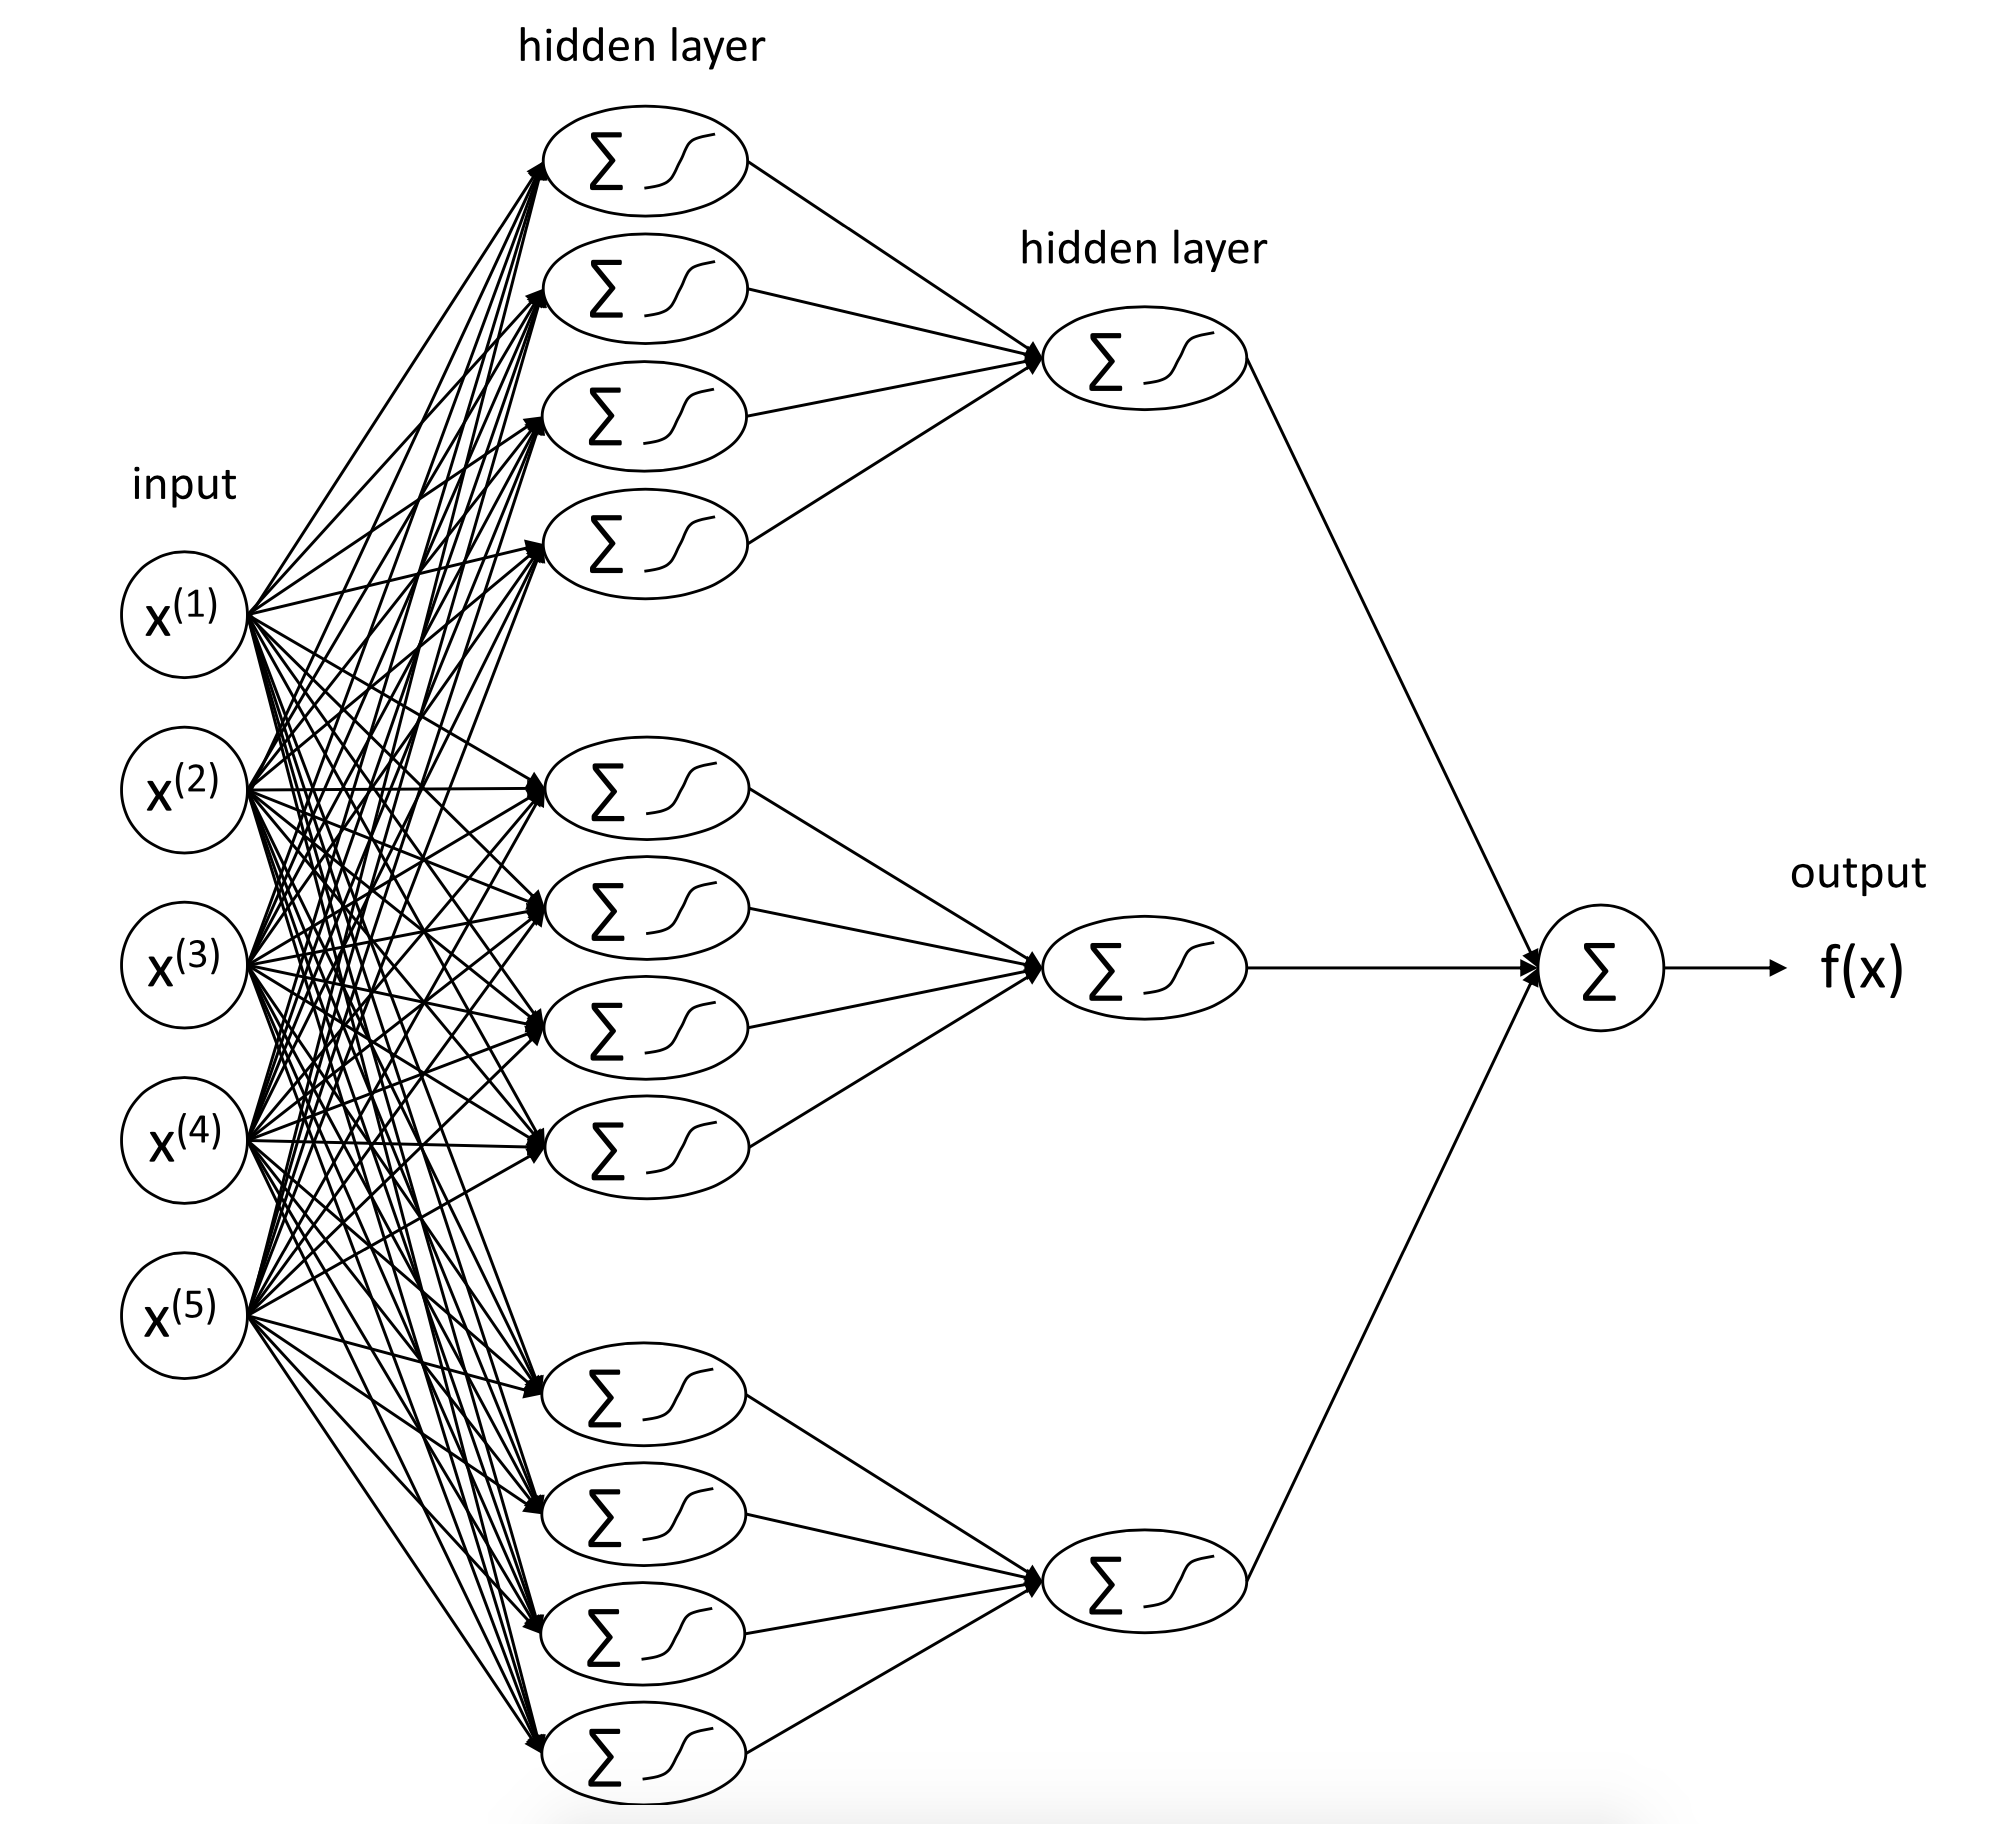
\includegraphics[width=0.75\textwidth]{Figures/DLNPR-Fig1}
	\caption{A not completely connected neural network $f:\SR^5\rightarrow \SR$ from $\calF_{M^*,d^*,d,\alpha}^{\text{(neural networks)}}$ with the structure $f(x) = \sum_{i=1}^3 \mu_i \cdot\sigma(\sum_{j=1}^4 \lambda_{i,j}\cdot\sigma(\sum_{v=1}^5 \theta_{i,j,v} \cdot x^{(v)}))$ (all weights with an index including zero neglected for a clear illustration). [Lifted from the paper]}
	\label{fig:DLNPR-1}
\end{figure}

For $l=0$, we define our space of hierarchical neural networks by 
\[\calH^{(0)} = \calF^{\text{(neural networks)}}_{M^*,d^*, d, \alpha} \]
For $l> 0$ we define recursively 
\begin{equation}
	\label{eq:DLNPR-6}
	\calH^{(l)} = \left\{h:\SR^d\rightarrow\SR: h(x) = \sum_{k=1}^K g_k(f_{1,k}(x),\dots, f_{d^*,k}(x))\text{ for some } g_k \in \calH^{(0)}\text{ and }f_{j,k} \in \calH^{(l-1)}\right\}
\end{equation}
The class $\calH^{(0)}$ is a set of neural networks with two hidden layers and a number of weights given by (\ref{eq;DLNPR-5}). From this, one can recursively conclude that for $l>0$, the class $\calH^{(l)}$ is a set of neural networks with $2\cdot l + 2$ hidden layers. This is illustrated below in Figure \ref{fig:DLNPR-Fig2}
\begin{figure}[htbp!]
	\centering
	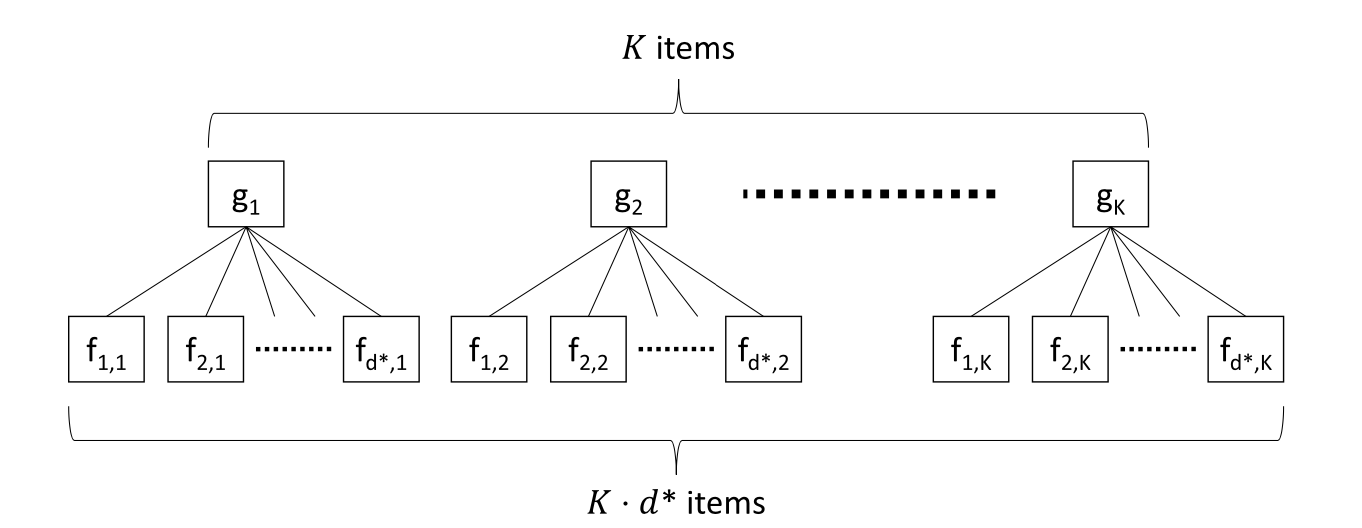
\includegraphics[width=0.75\textwidth]{Figures/DLNPR-Fig2}
	\caption{Illustration of the components of a function from $\calH^{(l)}$ [Lifted from the paper]}
	\label{fig:DLNPR-Fig2}
\end{figure}
Furthermore, let $N(\calH^{(l)})$ denote the number of linked two-layered networks from $\calF^{\text{(neural networks)}}_{M^*,d^*, d, \alpha}$ that define the functions from $\calH^{(l)}$. Then the following recursion holds: 
\begin{align*}
    N(\calH^{(0)}) &= 1,\\
    N(\calH^{(l)}) &= K + K\cdot d^* \cdot N(\calH^{(l-1)}),\hbox{ }\hbox{ }\hbox{ }\hbox{ }\hbox{ }l\in\SN
\end{align*}
which can be retraced following Figure \ref{fig:DLNPR-Fig2}. Above functions $g_1, \dots, g_K$ correspond to $K$ networks from $\calH^{(0)} =\calF^{\text{(neural networks)}}_{M^*,d^*, d, \alpha} $ and the $K\cdot d^*$ inner functions $f_{1,1},\dots, f_{d^*,K}$ originate from $\calH^{(l-1)}$, which leads to $K\cdot d^* \cdot N(\calH^{(l-1)})$ additional networks. 

Recursuve consideration yields
\begin{equation}
	\label{eq:DLNPR-7}
	N(\calH^{(l)}) = \sum_{t=1}^l {d^*}^{t-1}\cdot K^t + (d^*\cdot K)^l
\end{equation}
Consequently, a function from $\calH^{(l)}$ has at most 
\begin{equation}
	\label{eq:DLNPR-8}
	N(\calH^{(l)})\cdot W(\calF^{\text{(neural networks)}}_{M^*,d^*, d, \alpha})
\end{equation}
variable weights. Although this number of weights is exponential in the number of layers $l$, it can be controlled because a typical example of the technical systems which motivated Definition \ref{def:DLNPR-2} has only a moderate finite $l$. As explained in the definition, all typical assumptions for the regression function in the literature also correspond to a small $l$. 

Define $\tilde{m}_n$ as the least squares estimate 
\begin{equation}
	\label{eq:DLNPR-9}
	\tilde{m}_n(\cdot) = \arg \min_{h\in \calH^{(l)}} \frac{1}{n} \sum_{i=1}^n \left|Y_i - h(X_i)\right|^2
\end{equation}

For the result this needs to be truncated. Define the truncation operator $T_\beta$ with level $\beta > 0$ as 
\[T_\beta u = \begin{cases}
	u &\text{ if }|u|\leq \beta \\
	\beta \cdot \sign(u) &\text{ otherwise }
\end{cases}\]
Results requre a few additional properties on activation function, which are satisfied by many common activation functions (like the sigmoidal squasher) and they can be checked with arbitrary $N \in \SN_0$. Summarized in the next definition
\begin{definition}
	\label{def:DLNPR-3}
	A nondecresaing and Lipschitz continuous function $\sigma: \SR\rightarrow [0,1]$ is called \emph{$N$-admissable} if the following conditions hold
	\begin{enumerate}
		\item The function $\sigma$ is at least $N+1$ times differentiable with bounded derivatives. 
		\item A point $t_\sigma\in\SR$ exists where all derivatives up to the order $N$ of $\sigma$ are different from zero. 
		\item If $y > 0$, the relation $|\sigma(y) - 1| \leq \frac{1}{y}$ holds. If $y < 0$, the relation $|\sigma(y)| \leq \frac{1}{|y|}$ holds.
	\end{enumerate}
\end{definition}
\begin{theorem}[Main Result]
	\label{thm:DLNPR-1}
	Let $\{(X_i,Y_i)\}_{i=1}^n$ be independent and identically distributed random variables in $\SR^d\times\SR$ such that $\supp(X)$ is bounded and 
	\begin{equation}
		\label{eq:DLNPR-10}
		\mathbf{E}\exp(c_1 \cdot Y^2) < \infty, \footnote{This is basically saying that the moment generating function of $Y^2$ exists in some neighborhood around 0}
	\end{equation}
	for some constant $c_1 > 0$. Let $m$ be the corresponding regression function, which satisfies a $(p,C)$-smooth generalized hierarchical interaction model of order $d^*$ and finite level $l$ with $p = q+ s$ for some $q\in \SN_0$ and $s \in (0,1]$. Let $N\in \SN_0$ with $N\geq q$. Furthermore, assume that in Definition \ref{def:DLNPR-2}.b all partial derivatives of order less than or equal to $q$ of the functions $g_k, f_{j,k}$ are bounded. That is, assume that easch function $f$ satisfies
	\begin{equation}
		\label{eq:DLNPR-11}
		\max_{\substack{j_1,\dots,j_d \in \{0,1,\dots,q\}, \\ j_1+ \dots + j_d \leq q}} \left\Vert \frac{\partial^{j_1 + \dots + j_d}f}{\partial^{j_1}x^{(1)}\dots\partial^{j_d}x^{(d)}}\right\Vert \leq c_2
	\end{equation}
	and let all functions $g_k$ be Lipschitz continuous with Lipschitz constant $L> 0$ [which follows from (\ref{eq:DLNPR-11} if $q > 0$]. Let $\calH^{(l)}$ be defined as in (\ref{eq:DLNPR-6}) with $K, d, d^*$ as in the definition of $m$, $M^* = \left\lceil c_{56}\cdot n^{d^*}{2p + d^*}\right\rceil $. $\alpha = n^{c_{57}}$ for suffeciently large constants $c_{56}, c_{57} > 0$, and using an $N$-admissible $\sigma:\SR\rightarrow[0,1]$ according to Definition \ref{def:DLNPR-3}.Let $\tilde{m}_n$ be the least squares estimate defined by (\ref{eq:DLNPR-9}) and define $m_n = T_{c_3\log n}\tilde{m}_n$. Then 
	\[\mathbf{E}\int \left|m_n(x) - m(x)\right|^2 \mathbf{P}_X(dx) \leq c_4 \cdot \log^3(n) \cdot n^{-\frac{2p}{2p+d^*}}\]
	holds for suffeciently large $n$.
\end{theorem}
The authors include the following remarks on this main result
\begin{enumerate}
	\item For $p\geq 1$ and $C \geq 1$, the class of $(p,C)$-smooth generalized hierarchical interaction models of order $d^*$ satisfying the assumptions of the theorem contains all $(p,C)$-smooth functions, which depend on at most $d^*$ of its input components (because all functions in Def 2 can be chosen as projections). So, the rate of convergence in Theorem \ref{thm:DLNPR-1} is optimal up to some logarithmic factor, according to Stone (1982). 
	\item Some parameters of the estimate $m_n$, like $l, K$, or $d^*$ can be uknown in practice. They then would have to be chosen in a data dependent way. This has been studied in the literature apparently.
	\item Equation (\ref{eq:DLNPR-10}) in above theorem prevents heavy tails and ensure that the distribution of $Y$ is suffeciently concentrated in order to allow good estimates. 
\end{enumerate}
\begin{corollary}
	Suppose $\{(X_i,Y_i)\}_{i=1}^n$ is an i.i.d sample with values in $\SR^d\times\SR$ such that the support of $X$ is bounded and $\mathbf{E}\exp(c_1\cdot Y^2) < \infty$ for some constant $c_1 > 0$. Suppose the corresponding regression function $m$ satisfies a $(2,C)$-smooth generalized hierarchical interaction model of order 2 and finite level 0. Further assume that in Definition \ref{def:DLNPR-2}.b all partial derivatives of order $\leq 1$ of $g_k, f_{j,k}$ are bounded. Take $M^* = \left\lceil c_{56}n^{\frac{1}{3}}\right\rceil$. Use $\sigma(z) = \frac{1}{1+ \exp(-z)}$ and $\tilde m_n$ and $m_n$ as defined in Theorem \ref{thm:DLNPR-1}. Then
	\[\mathbf{E}\int \left|m_n(x) - m(x) \right|^2 \mathbf{P}_X(dx) \leq c_4\cdot\log^3(n)\cdot n^{-\frac{2}{3}},\footnote{Stringent conditions, but that is a wicked rate of convergence}\]
	holds for sufficiently large \(n\).
\end{corollary}
\begin{proof}
	Using notation from Theorem \ref{thm:DLNPR-1}, can choose $N = 1 = 1$. The sigmoidal squasher $\sigma$ is 1-admissible. Then the application of Theorem \ref{thm:DLNPR-1} implies the corollary.
\end{proof}

\subsection{Application to Simulated Data}

Section compares the neural net to an adaptive $k$-nearest neighbors appraoch as interpolation with radial basis function (\emph{RBF}). 
The paramaters $l, K, d^*, M^*$ of the neural network estimate (\emph{neural-x}) defined in Theorem \ref{thm:DLNPR-1}. To solve the least squares problem in (\ref{eq:DLNPR-9}). To solve the least squares problem use the quasi-Newton method of the function \emph{fminunc} in \emph{MATLAB} to approximate a solution.

Also compare this neural network estimate, which is characterized by the data-dependent choice of its structure and not completely connected neurons, to more ordinary fully connected neural networks with predefined numbers of layers but adaptively chosen numbers of neurons per layer.

Estimate outpreforms the other approaches in the three typical examples for generalized hierarchical interaction models. In these cases, the relative improvement of the estimate is larger with a larger sample size, which is an indicator of a better rate of convergence.

In some more extreme cases, this paper's approach is not always the best, though it still preforms will in some situations. In any case though, the results from simulation are promising. 

\subsection{Proofs}

Won't be covered in notes, but the proofs are given in section four of the paper and would be a good idea to examine.


